\part{Basics}
\frame{\partpage}

\section{Why Buy a Big Computer?}

\begin{frame}{Basics: Why Buy a Big Computer?}

What types of big problem might require a ``Big Computer''?

\begin{description}
\pause
\item[\textit{Compute Intensive:}]{A single problem requiring a large amount of computation.}
\pause
\item[\textit{Memory Intensive:}]{A single problem requiring a large amount of memory.}
\pause
\item[\textit{Data Intensive:}]{A single problem operating on a large amount of data.}
\pause
\item[\textit{High Throughput:}]{Many unrelated problems to be executed in bulk.}
\end{description}
\end{frame}

\begin{frame}{Basics: Compute Intensive Problems}
\begin{itemize}
\item{Distribute the \alert{work} for a \alert{single problem} across multiple CPUs to reduce the execution time as far as possible.}
\pause
\item{Program workload must be \emph{parallelised}:}
\begin{description}
\item{Parallel programs split into copies (processes or threads).}
\item{Each process/thread performs a part of the work on its own CPU, concurrently with the others.}
\item{A well-parallelised program will fully exercise as many CPUs as there are processes/threads.}
\end{description}
\pause
\item{The CPUs typically need to exchange information rapidly, requiring specialized communication hardware.}
\pause
\item{Many use cases from Physics, Chemistry, Engineering, Astronomy, Biology...}
\item{The traditional domain of \alert{HPC} and the \alert{Supercomputer}.}
\end{itemize}
\end{frame}

\begin{frame}{Basics: Scaling \& Amdahl's Law}
\begin{itemize}
\item{\alert{Using more CPUs is not necessarily faster.}}
  \pause
\item{Typically parallel codes have a \alert{scaling limit}.}
\item{Partly due to the system overhead of managing more copies, but also to more basic constraints;}
\pause
\item{Amdahl's Law (idealized):}
\[
S(N)=\frac{1}{\left(1-p+\frac{p}{N}\right)}
\]
where \begin{align*}S(N)&\text{ is the fraction by which the program has sped up}\\&\text{ relative to $N=1$}\\
p&\text{ is the fraction of the program which can be parallelized}\\
N&\text{ is the number of CPUs.}
\end{align*}
\end{itemize}
\end{frame}

\begin{frame}{Basics: Amdahl's Law}
\centerline{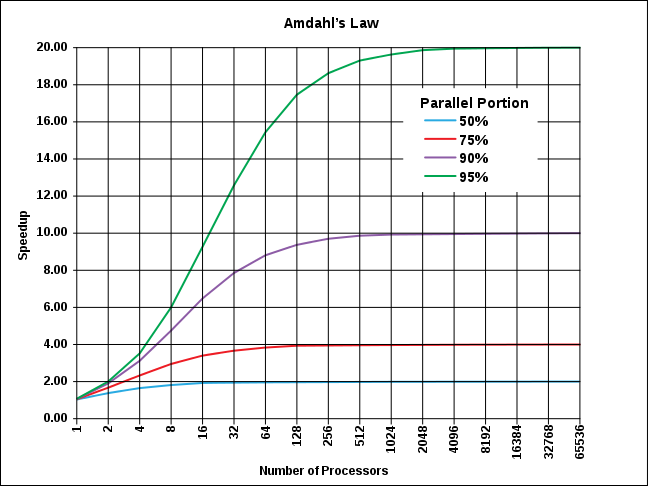
\includegraphics[width=0.75\textwidth]{imgs/AmdahlsLaw.png}}%
\rightline{\tiny http://en.wikipedia.org/wiki/File:AmdahlsLaw.svg}
\smallskip
\end{frame}

\begin{frame}{The Bottom Line}
\begin{itemize}
\item{Parallelisation requires effort:}
\begin{itemize}
\item{There are libraries to help (e.g. \alert{OpenMP}, \alert{MPI}).}
\item{First optimise performance on one CPU, then make $p$ as large as possible.}
\end{itemize}
\pause
\item{The scaling limit: eventually using more CPUs becomes \alert{detrimental} instead of helpful.}
\end{itemize}
\end{frame}

\begin{frame}{Basics: Data Intensive Problems}
\begin{itemize}
\item{Distribute the \alert{data} for a \alert{single problem} across multiple CPUs to reduce the overall execution time.}
\pause
\item{The \emph{same} work may be done on each data segment.}
\pause
\item{Rapid movement of data to and from disk is more important than inter-CPU communication.}
\pause
\item{\alert{Big Data} problems of great current interest -}
\item{Hadoop/MapReduce}
\item{Life Sciences (genomics) and elsewhere.}
\end{itemize}
\end{frame}

\begin{frame}{Basics: High Throughput}
\begin{itemize}
\item{Distribute \alert{independent}, \alert{multiple problems} across multiple CPUs to reduce the overall execution time.}
\pause
\item{Workload is trivially (or \emph{embarrassingly}) parallel:}
\begin{itemize}
\item[$\ast$]{Workload breaks up naturally into \emph{independent} pieces.}
\item[$\ast$]{Each piece is performed by a separate process/thread on a separate CPU (concurrently).}
\item[$\ast$]{\alert{Little or no inter-CPU communication}.}
\end{itemize}
\pause
\item{Emphasis is on throughput over a period, rather than on performance on a single problem.}
\pause
\item{Compute intensive capable $\Rightarrow$ high throughput capable}
\pause
\item{\color{red}Compute intensive capable $\not\Leftarrow$ high throughput capable} 
\end{itemize}
\end{frame}

\begin{frame}{Basics: Memory Intensive Problems}
\begin{itemize}
\item{Require aggregation of large memory into a \alert{single system image} (i.e.\ a single computer running Linux).}
%\pause
%\begin{description}
%\item{\alert{NB Memory (fast, volatile) not disk (slow, non-volatile).}}
%\end{description}
\pause
\item{Technically more challenging to build machines (very fast, low latency interconnection between \alert{all} CPUs and \alert{all} memory).}
\pause
\item{Coding/porting easier (memory appears seamless).}
\pause
\item{Optimisation harder (memory is actually highly nonuniform).}
\pause
\item{Historically, the arena of large \alert{SGI} systems.}
\pause
\item{Nowadays, similar complexity inside single commodity servers.}
\end{itemize}
\end{frame}

\section{Inside a Modern Computer}
\begin{frame}{Basics: Inside a Modern Computer}{CPUs in a box}
\only<1-7>{%
\begin{itemize}
\item<1-7>{Today's commodity servers already aggregate both CPUs and memory to make a single system image in a single box.}
\item<2-7>{Even small computers now have multiple CPU cores per socket\hfill\\
\visible<3-7>{\alert{$\implies{}$each socket is a Symmetric Multi-Processor (SMP).}}}
\item<4-7>{Larger computers have multiple sockets (each with local memory):\hfill\\
{}\qquad all CPU cores (unequally) share the node memory\hfill\\
{}\qquad \visible<5-7>{$\implies{}$the node is a \alert{shared memory} multiprocessor}\\
{}\qquad \visible<6-7>{with Non-Uniform Memory Architecture (\alert{NUMA})}\\
{}\qquad \visible<7>{but users still see a single computer (\alert{single system image}).}}
\end{itemize}
}%
\end{frame}

\begin{frame}{Basics: Inside a Modern Computer}{CPUs in a box}
\centerline{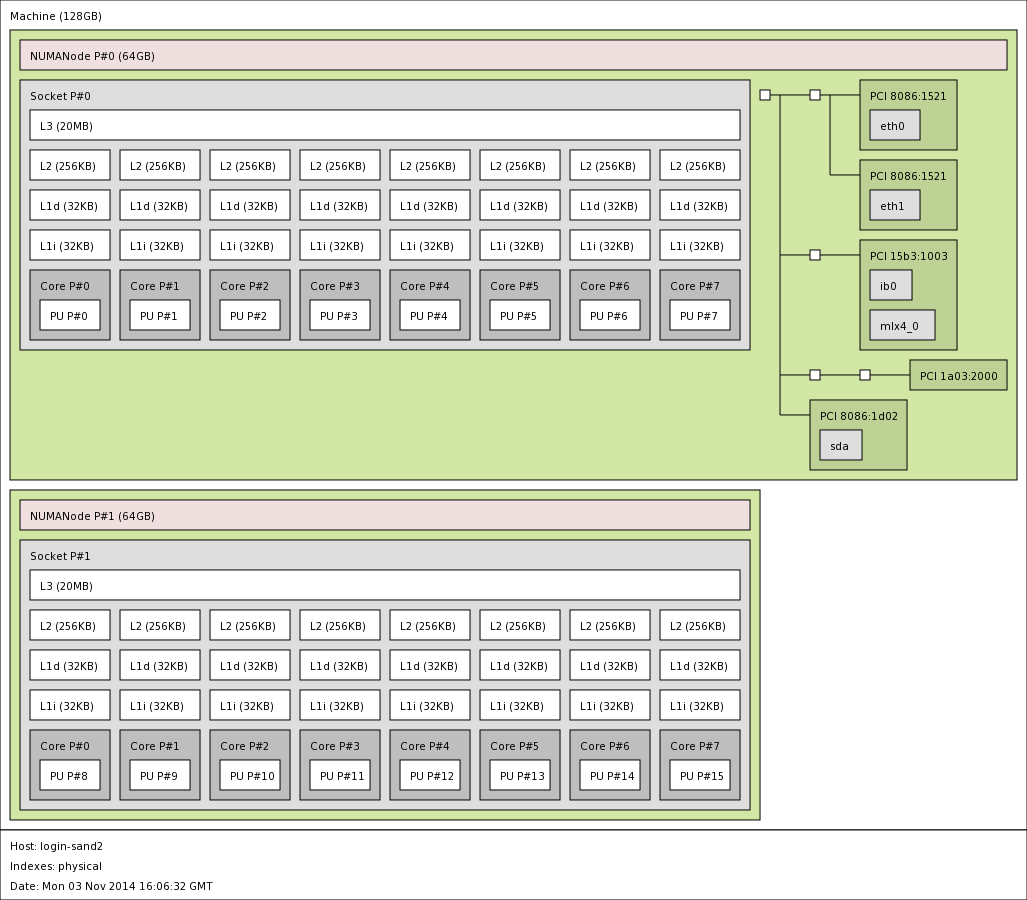
\includegraphics[width=0.8\textwidth]{imgs/lstopo.png}}
\end{frame}

\section{How to Build a Supercomputer}
\begin{frame}{Basics: How to Build a Supercomputer}
\only<1,2>{\begin{itemize}
\item{A supercomputer aggregates contemporary CPUs and memory to obtain increased computing power.}
\pause
\item{Usually today these are \alert{clusters}.}
\end{itemize}}
\only<3->{\begin{enumerate}
\item{Take some (multicore) CPUs plus some memory.}
\begin{itemize}
\item<4->{Could be an off-the-shelf server, or something more special.}
\item<5->{A NUMA, shared memory, multiprocessor building block: a \alert{node}.}
\end{itemize}
\end{enumerate}
}
\end{frame}

\begin{frame}{Basics: How to Build a Supercomputer}
\begin{tabular}{ll}
\parbox[c]{0.5\textwidth}{\begin{enumerate}
\setcounter{enumi}{1}
\item{Connect the nodes with one or more \alert{networks}. E.g.}
\begin{description}
\item[Gbit Ethernet:]{\alert{100 MB/sec}}
\item[Omni-Path:]{\alert{10 GB/sec}}
\end{description}
\pause
\null\par
Faster network is for \alert{inter-CPU communication across nodes}.\par
Slower network is for \alert{management} and \alert{provisioning}.\par
\alert{Storage} may use either.
\end{enumerate}}
&\vbox to 0pt{\vss\vskip 0.25cm\leftline{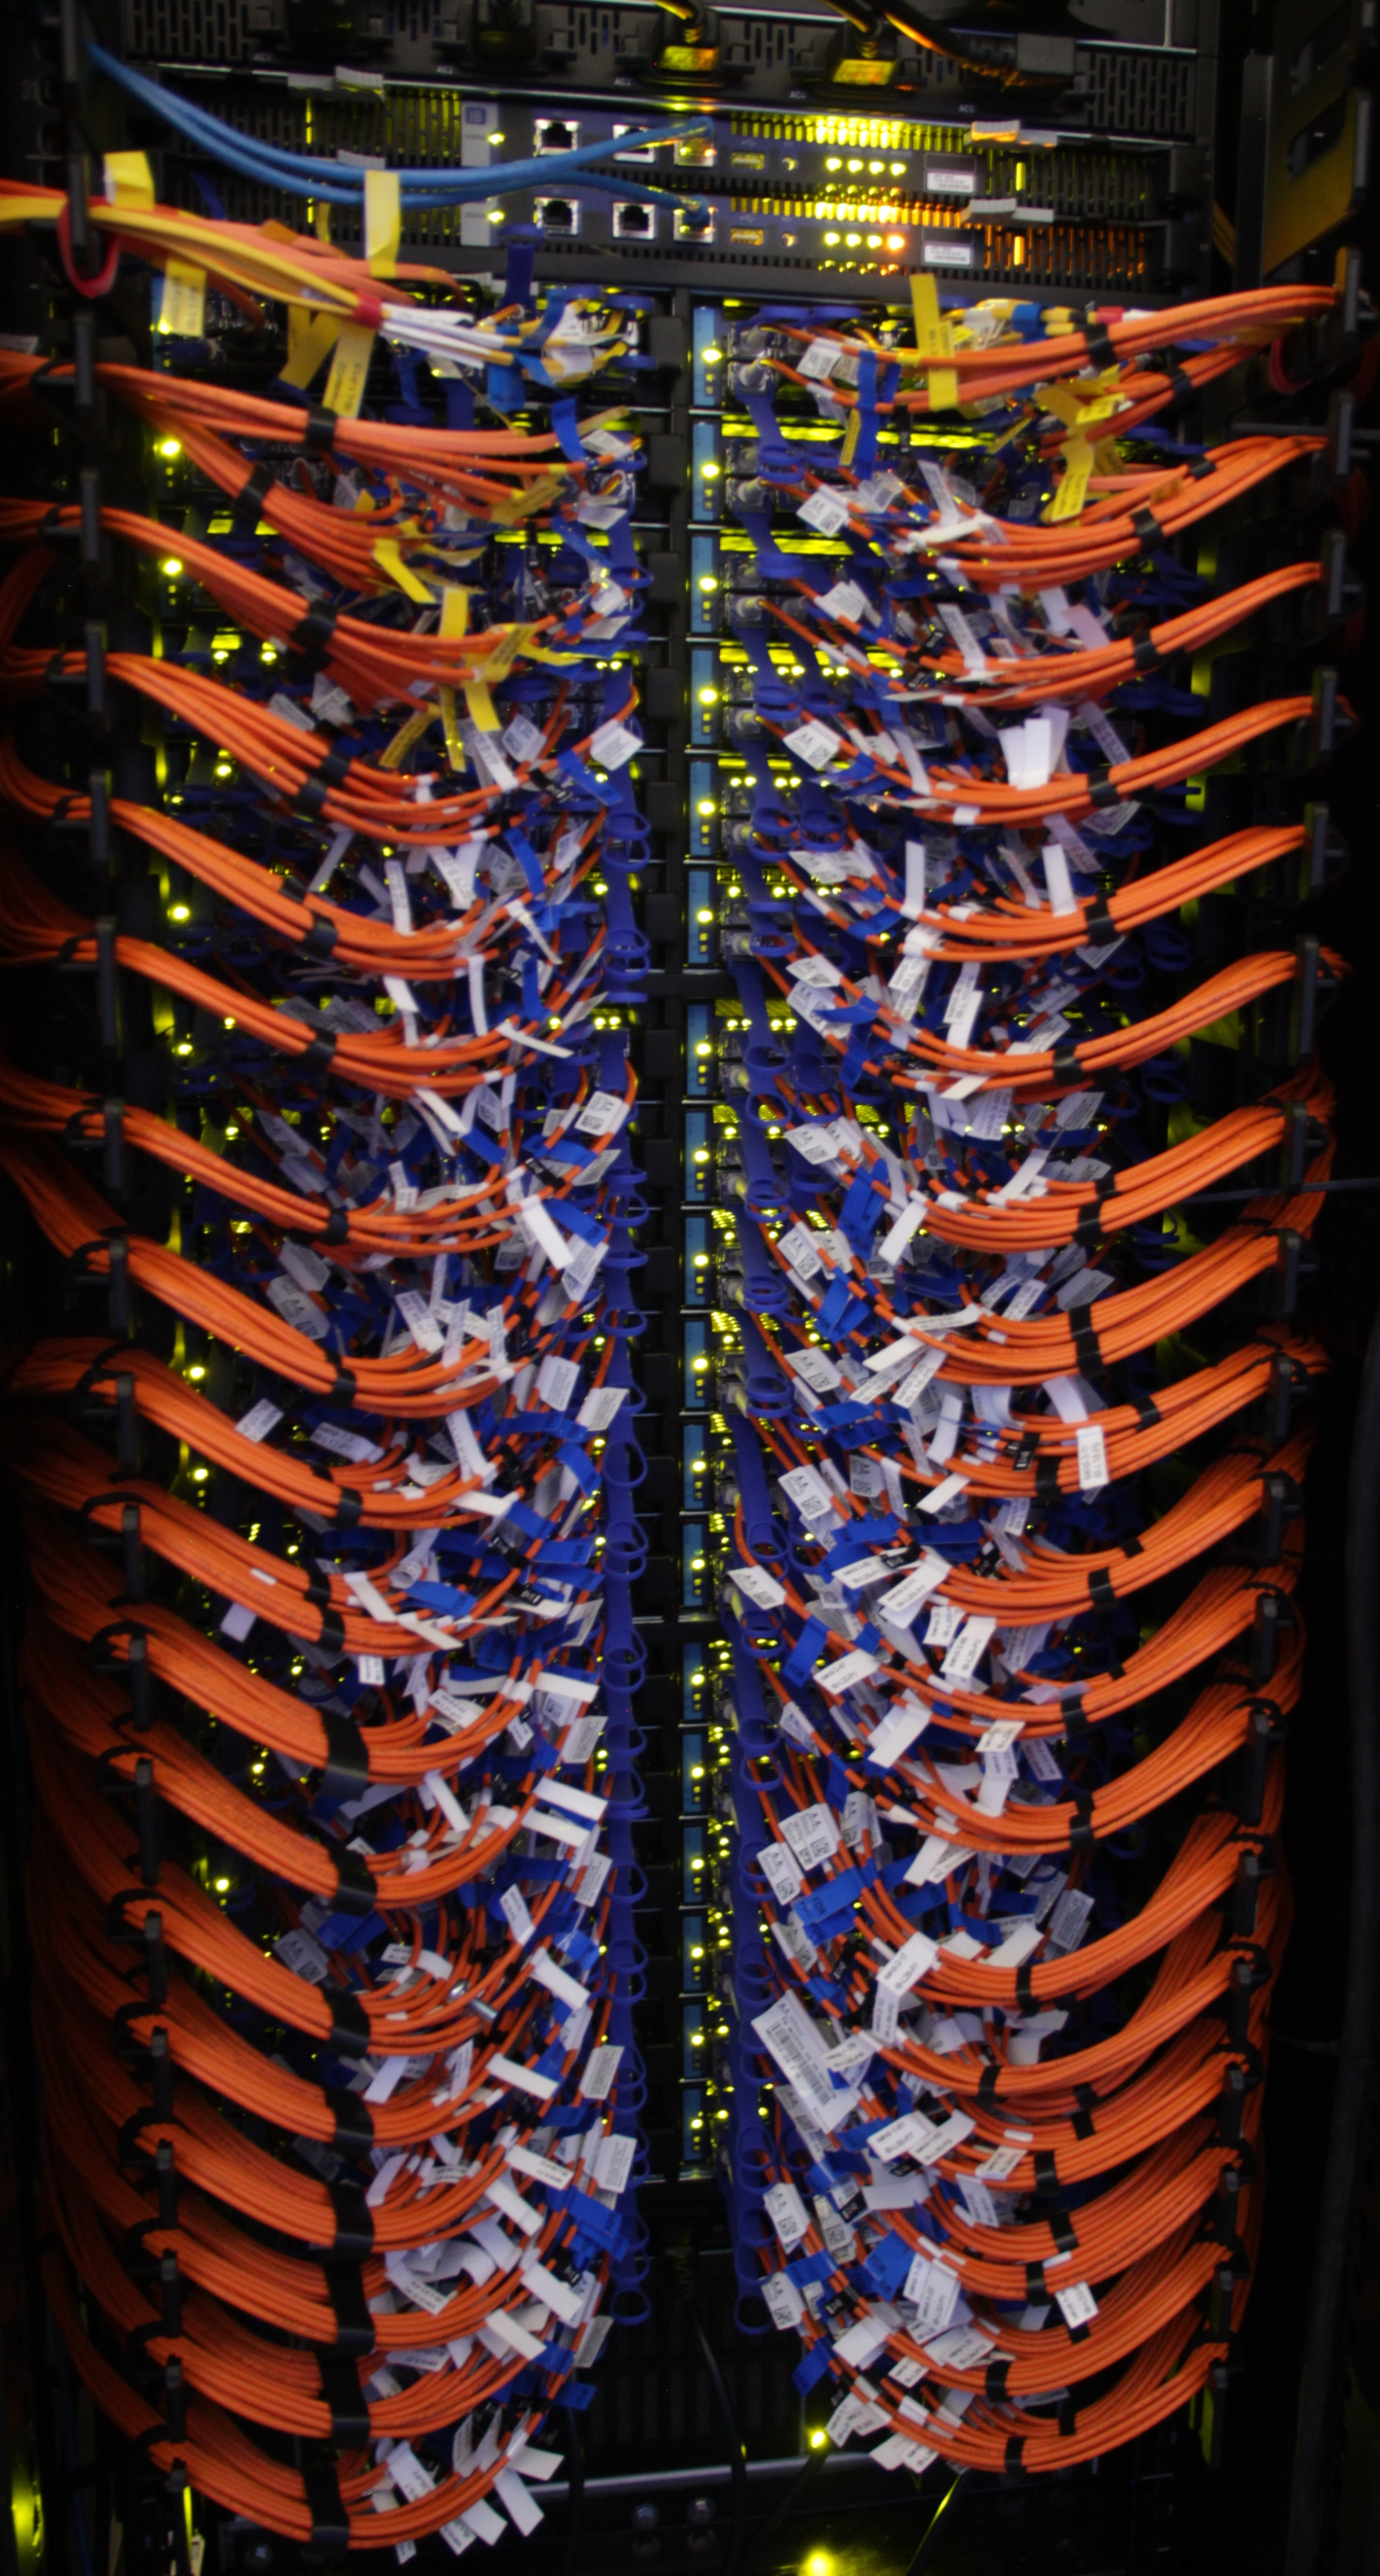
\includegraphics[height=0.85\textheight]{imgs/coreib.jpg}}\vss}\\
\end{tabular}
\end{frame}

\begin{frame}{Basics: How to Build a Supercomputer}
\begin{enumerate}
\setcounter{enumi}{2}
\item{Logically bind the nodes}
\begin{itemize}
\item{Clusters consist of distinct nodes (i.e. separate Linux computers)\hfill\\
on common private network(s) and controlled centrally.}
\begin{itemize}
\item[$\ast$]{Private networks allow CPUs in different nodes to communicate.}
\pause
\item[$\ast$]{Clusters are \alert{distributed memory} machines:\hfill\\
\alert{Each process/thread sees only its local node's CPUs and memory (without help).}}
\pause
\item[$\ast$]{\color{red}Each process/thread must fit within a single node's memory.}
\end{itemize}
\pause
\item{More expensive machines logically bind nodes into a single system\hfill\\
{}\qquad i.e. CPUs \alert{and} memory.}
\begin{itemize}
\item[$\ast$]{E.g.\ SGI UV.}
\item[$\ast$]{Private networks allow CPUs to see CPUs and memory in other nodes.}
\pause
\item[$\ast$]{These are \alert{shared memory} machines.}
\item[$\ast$]{Logically a single system - 1 big node - but very non-uniform.}
\item[$\ast$]{A single process can span the entire system.}
\end{itemize}
\end{itemize}
\end{enumerate}
\end{frame}

\section{Programming a Multiprocessor Machine}
\begin{frame}{Basics: Programming a Multiprocessor Machine}
\only<1-3>{\begin{itemize}
\item{Non-parallel (serial) code}
\begin{itemize}
\item[$\ast$]{\alert{For a single node as for a workstation.}}
\pause
\item[$\ast$]{Typically \alert{run as many copies per node as CPUs}, assuming node memory is sufficent.}
\pause
\item[$\ast$]{\alert{Replicate across multiple nodes.}}
\end{itemize}
\end{itemize}}
\only<4->{\begin{itemize}
\item{Parallel code}
\begin{itemize}
\item<5->[$\ast$]{\alert{Shared memory methods within a node.}\hfill\\
E.g. pthreads, OpenMP.}
\item<6->[$\ast$]{\alert{Distributed memory methods spanning multiple nodes.}\hfill\\
Message Passing Interface (MPI).}
\end{itemize}
\end{itemize}}
\end{frame}

\section{Summary}

\begin{frame}{Basics: Summary}
  \begin{itemize}
  \item<1->{\alert{Why have a supercomputer?}}
  \begin{itemize}\item<2->{Big single problems, many problems, Big Data.}\end{itemize}
  \item<3->{Most current supercomputers are \alert{clusters} of separate \alert{nodes}.}
  \item<4->{Each node has \alert{multiple CPUs} and \alert{non-uniform shared memory}.}
  \item<5->{\alert{Parallel} code uses shared memory (\alert{pthreads/OpenMP}) within a node, distributed memory (\alert{MPI}) spanning multiple nodes.}
  \item<6->{\alert{Non-parallel} code uses the memory of one node, but may be copied across many.}
  \end{itemize}
  
\end{frame}

\part{HPC Facilities}
\frame{\partpage}

\section{CSD3}
\begin{frame}{CSD3 - University of Cambridge}
\begin{itemize}
\item{Cambridge Service for Data Driven Discovery}
\pause
\medskip
\item{\alert{Peta4 --- Intel CPU cluster}}
\pause
\item{\alert{Wilkes2 --- NVIDIA GPU cluster}}
\pause
\medskip
\item{Hadoop-based data analytic platform}
\item{Burst buffer}
\item{Industry users and collaborators through CORE.}
\end{itemize}
\end{frame}

\section{Peta4-Skylake}
\begin{frame}{Peta4-Skylake}
\begin{itemize}
\item{Each compute node:}
\begin{itemize}
\item[$\ast$]{\only<1>{2x16 cores, Intel Skylake 2.6 GHz}\only<2->{{\color{red}32 CPUs}}}
\item[$\ast$]{\only<1>{$192\,\text{GB}$ or $384\,\text{GB}$ RAM}\only<2->{{\color{red}$6\,\text{GB}$ or $12\,\text{GB}$ per CPU}}}
\item[$\ast$]{\only<1>{$100\,\text{Gb/sec}$ Omni-Path}\only<2->{\color{red}$10\,\text{GB/sec}$ (for MPI and storage)}}
\end{itemize}
\item{768 compute nodes}
\item{8 login nodes (\alert{login-cpu.hpc.cam.ac.uk})}
\end{itemize}
\end{frame}

\section{Coprocessors --- GPUs etc}
\begin{frame}{Coprocessors --- GPUs etc}
  \begin{itemize}
  \item{CPUs are \alert{general purpose}}
    \pause
  \item{Some types of parallel workload fit \alert{vector} processing well:}
    \begin{itemize}
    \item{Single Instruction, Multiple Data (SIMD)}
    \item{\emph{Think pixels on a screen}}\pause
    \item{GPUs specialise in this type of work}\pause
      \item{Also competitor many-core architectures such as the Intel Phi}
    \end{itemize}
\end{itemize}
\end{frame}

\section{Wilkes2-GPU}
\begin{frame}{Wilkes2-GPU}
\begin{itemize}
\item{Each compute node:}
\begin{itemize}
\item[$\ast$]{\only<1>{$4\times\text{NVIDIA P100 GPU}$}\only<2->{\color<2->{red}4 GPUs}}
\item[$\ast$]{\only<1>{1x12 cores, Intel Broadwell 2.2 GHz}\only<2->{{\color{red}12 CPUs}}}
\item[$\ast$]{\only<1>{$96\,\text{GB}$ RAM}\only<2->{{\color{red}$96\,\text{GB}$ RAM}}}
\item[$\ast$]{\only<1>{$100\,\text{Gb/sec}$ (4X EDR) Infiniband.}\only<2->{\color{red}$10\,\text{GB/sec}$ (for MPI and storage)}}
\end{itemize}
\item{90 compute nodes.}
\item{8 login nodes (\alert{login-gpu.hpc.cam.ac.uk}).}
\end{itemize}
\end{frame}

\section{Peta4-KNL}
\begin{frame}{Peta4-KNL (Intel Phi)}
\begin{itemize}
\item{Each compute node:}
\begin{itemize}
\item[$\ast$]{\only<1>{64 cores, Intel Phi 7210}\only<2->{{\color{red}256 CPUs}}}
\item[$\ast$]{\only<1>{$96\,\text{GB}$ RAM}\only<2->{{\color{red}$96\,\text{GB}$ RAM}}}
\item[$\ast$]{\only<1>{$100\,\text{Gb/sec}$ Omni-Path}\only<2->{\color{red}$10\,\text{GB/sec}$ (for MPI and storage)}}
\end{itemize}
\item{342 compute nodes}
\item{Shared login nodes with Peta4-Skylake}
\end{itemize}
\end{frame}


\begin{frame}{HPCS Production Cluster Schematic}
\centerline{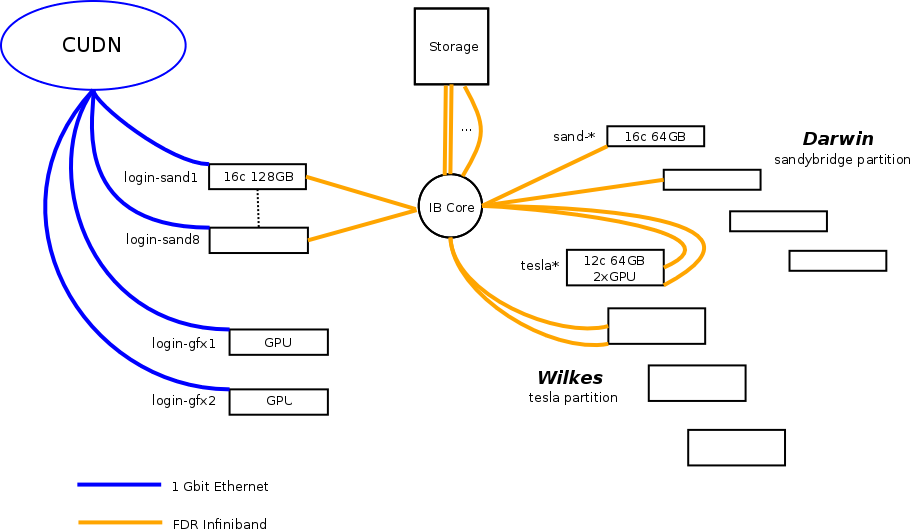
\includegraphics[width=0.95\textwidth]{imgs/cluster.png}}%
\end{frame}

\section{Storage}
\begin{frame}{Cluster Storage}
  \begin{itemize}
\item{CSD3 uses the Lustre cluster filesystem:}
  \begin{itemize}
\item[$\ast$]{Very scalable, high bandwidth.}
\item[$\ast$]{Multiple RAID6 back-end disk volumes.}
\item[$\ast$]{Multiple object storage servers.}
\item[$\ast$]{Single metadata server.}
\item[$\ast$]{Tape-backed HSM on newest filesystems.}
\item[$\ast$]{\alert{$12\,\text{GB/sec}$ overall read or write.}}
\item[$\ast$]{\alert{Prefers big read/writes over small.}}
\end{itemize}
\end{itemize}
\end{frame}

\section{Obtaining an Account and Support}
\begin{frame}{Obtaining an Account and Support}
\begin{itemize}
\item{Please contact the NPL IT Service Desk:}
  \begin{itemize}
\item{\alert{itservicedesk@npl.co.uk}}
\item{Room F12-CS1}
\item{Tel.~6000}
  \end{itemize}
  \pause
  \item{Second line support is provided by the Cambridge RCS.}
\end{itemize}
\end{frame}

\part{Using HPC}
\frame{\partpage}

\section{Connecting}
\begin{frame}{Using HPC: Connecting}
\begin{itemize}
\item SSH secure protocol only.\hfill\\
\visible<2->{\alert{Supports login, file transfer, remote desktop\ldots}}
\end{itemize}
\end{frame}

\subsection{Windows Clients}
\begin{frame}{Connecting: Windows Clients}
\begin{itemize}
\item<1-5> putty, pscp, psftp\hfill\\
\alert{\small http://www.chiark.greenend.org.uk/~sgtatham/putty/download.html}
\item<2-5> WinSCP\hfill\\
\alert{\small http://winscp.net/eng/download.php}
\item<3-5> TurboVNC \alert{\small (remote desktop, 3D optional)}\hfill\\
\alert{\small http://sourceforge.net/projects/turbovnc/files/}
\item<4-5> Cygwin \visible<5>{\alert{\small (provides an application environment similar to Linux)}}\hfill\\
\alert{\small http://cygwin.com/install.html}\hfill\\
\visible<5>{\alert{\small Includes X server for displaying graphical applications running remotely.}}
\item<6> MobaXterm\hfill\\
\alert{\small http://mobaxterm.mobatek.net/}
\end{itemize}
\end{frame}

\subsection{Linux/MacOSX/UNIX Clients}
\begin{frame}{Connecting: Linux/MacOSX/UNIX Clients}
\begin{itemize}
\item {\color<2->{red}ssh}, scp, sftp, {\color<2->{red}rsync}\hfill\\
\alert{\small Installed (or installable).}
\item<3-> TurboVNC \alert{\small (remote desktop, 3D optional)}\hfill\\
\alert{\small http://sourceforge.net/projects/turbovnc/files/}
\item<4-> On MacOSX, install \alert{XQuartz} to display remote graphical applications.\hfill\\
\alert{\small http://xquartz.macosforge.org/landing/}
\end{itemize}
\end{frame}

\subsection{Login}
\begin{frame}{Connecting: Login}
\begin{itemize}
\item From graphical clients:\hfill\\
Host: \alert{minerva-login1.npl.co.uk}\hfill\\
Username: \alert{\textbf{npl$\backslash$abc123}} (your NPL AD account name)
\pause
\item From Linux/MacOSX/UNIX (or Cygwin):\hfill\\\medskip
  \alert{ssh -Y \textbf{npl$\backslash\backslash$abc12}@minerva-login1.npl.co.uk}\hfill\\\medskip
  Note the double backslash --- this is because UNIX command interpreters treat $\backslash$ as special.
\end{itemize}
\end{frame}

\begin{frame}{Connecting: First time login}
\begin{itemize}
\item{The first connection to a particular hostname produces the following:}
\begin{semiverbatim}\tiny
The authenticity of host 'minerva-login1.npl.co.uk (139.143.201.10)' can't be established.


ECDSA key fingerprint is {\color<2->{red}SHA256:k/eB+LjcAfQW56XCzK9QptT0wVWF7j3a/CPxPRd7+lE}.

ECDSA key fingerprint is {\color<2->{red}MD5:18:9a:97:e2:87:4c:07:60:cb:43:46:f2:bb:d8:3d:01}.


Are you sure you want to continue connecting (yes/no)? {\color<3->{red}yes}

Warning: Permanently added 'minerva-login1.npl.co.uk (139.143.201.10)' (ECDSA) to the list of known hosts.
\end{semiverbatim}
\smallskip\item{\alert{One should always check the fingerprint before typing ``yes''.}}
\item{Graphical SSH clients \emph{should} ask a similar question.}
\item{Designed to detect fraudulent servers.}
\end{itemize}
\end{frame}

\begin{frame}[fragile]{Connecting: First time login}
\begin{itemize}
\item{Exercise 1 - Log into your Minerva account.}
  \pause
  \item{Exercise 2 - Simple command line operations.}
\end{itemize}
\end{frame}

\subsection{File Transfer}
\begin{frame}{Connecting: File Transfer}
\begin{itemize}
\item With graphical clients, connect as before and drag and drop.
\pause
\item From Linux/MacOSX/UNIX (or Cygwin):\hfill\\
\alert{\footnotesize rsync -av \textbf{old\_directory/} npl$\backslash\backslash$abc12@minerva-login1.npl.co.uk:hpc-work/new\_directory}\hfill\\
copies contents of old\_directory to $\tilde{}\text{/hpc-work/new\_directory}$.\hfill\\\smallskip
\pause
\alert{\footnotesize rsync -av \textbf{old\_directory} npl$\backslash\backslash$abc12@minerva-login1.npl.co.uk:hpc-work/new\_directory}\hfill\\
copies old\_directory (and contents) to $\tilde{}\text{/hpc-work/new\_directory/old\_directory}$.\hfill\\
\pause
\begin{itemize}
\item[$\ast$]Rerun to update or resume after interruption.
\item[$\ast$]All transfers are checksummed.
\item[$\ast$]For transfers in the opposite direction, place the remote machine as the first argument.
\end{itemize}
\pause
\item{Exercise 3 - File transfer.}
\end{itemize}
\end{frame}

\subsection{Remote Desktop}
\begin{frame}[fragile]{Connecting: Remote Desktop}
\begin{itemize}
\item First time starting a remote desktop:
\begin{semiverbatim}
\footnotesize
[sjr20@login-a-1 ~]\$ vncserver

You will require a password to access your desktops.

Password: 
Verify:   
Would you like to enter a view-only password (y/n)? n

New 'login-a-1:99 (sjr20)' desktop is login-a-1:{\color{red}99}

Starting applications specified in /home/sjr20/.vnc/xstartup
Log file is /home/sjr20/.vnc/login-a-1:99.log
\end{semiverbatim}
\item{NB Choose a \alert{different} password for VNC.}
\item{The VNC password protects your desktop from other users.}
\item{Remember the unique display number ({\color{red}99} here) of your desktop.}
\end{itemize}
\end{frame}

\begin{frame}[fragile]{Connecting: Remote Desktop}
\begin{itemize}
\item Remote desktop already running:
\begin{semiverbatim}
\footnotesize
[sjr20@login-a-1 ~]\$ vncserver -list

TigerVNC server sessions:

X DISPLAY #     PROCESS ID
:99             130655
\end{semiverbatim}
\smallskip\item Kill it:
\begin{semiverbatim}
\footnotesize
[sjr20@login-a-1 ~]\$ vncserver -kill :99
Killing Xvnc process ID 130655
\end{semiverbatim}
\smallskip\item\alert{Typically you only need {\color{red}one} remote desktop.}
\item\alert{Keeps running until killed, or the node reboots.}
\end{itemize}
\end{frame}

\begin{frame}[fragile]{Connecting: Remote Desktop}
\begin{itemize}
\item To connect to the desktop from Linux:\\\hfill\break
{\scriptsize
\alert{vncviewer -via npl$\backslash\backslash$abc12@minerva-login1.npl.ad.local localhost:99}}
\smallskip
\item{The display number \alert{99} will be different in general and unique to each desktop.}
\item{You will be asked firstly for your AD login password, and secondly for your VNC password.}
\item{\alert{Press F8 to bring up the control panel.}}
\pause
\item{Exercise 4 - Remote desktop (from Windows)}
\end{itemize}
\end{frame}


%\begin{frame}{TurboVNC Session}
%\begin{center}
%\centerline{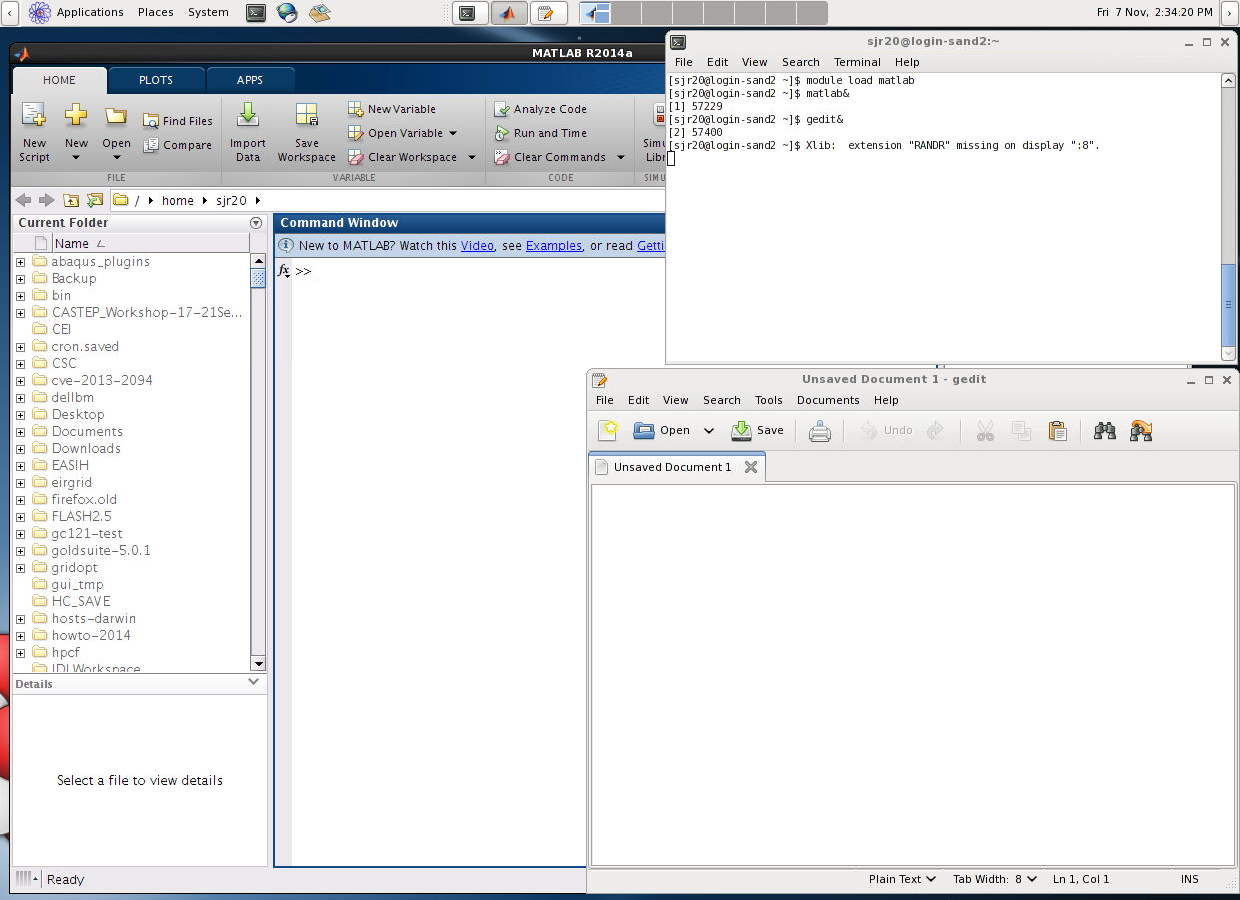
\includegraphics[width=0.85\textwidth]{imgs/linux-turbovnc.png}}
%\end{center}
%\end{frame}

%\begin{frame}{Linux TurboVNC Control Panel}
%\begin{center}
%\centerline{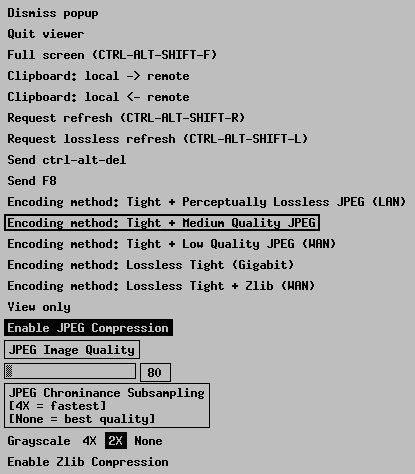
\includegraphics[height=0.8\textheight]{imgs/linux-turbovnc-F8.png}}
%\end{center}
%\end{frame}

\begin{frame}{Connecting: Remote Desktop (MobaXterm)}
\begin{center}
\centerline{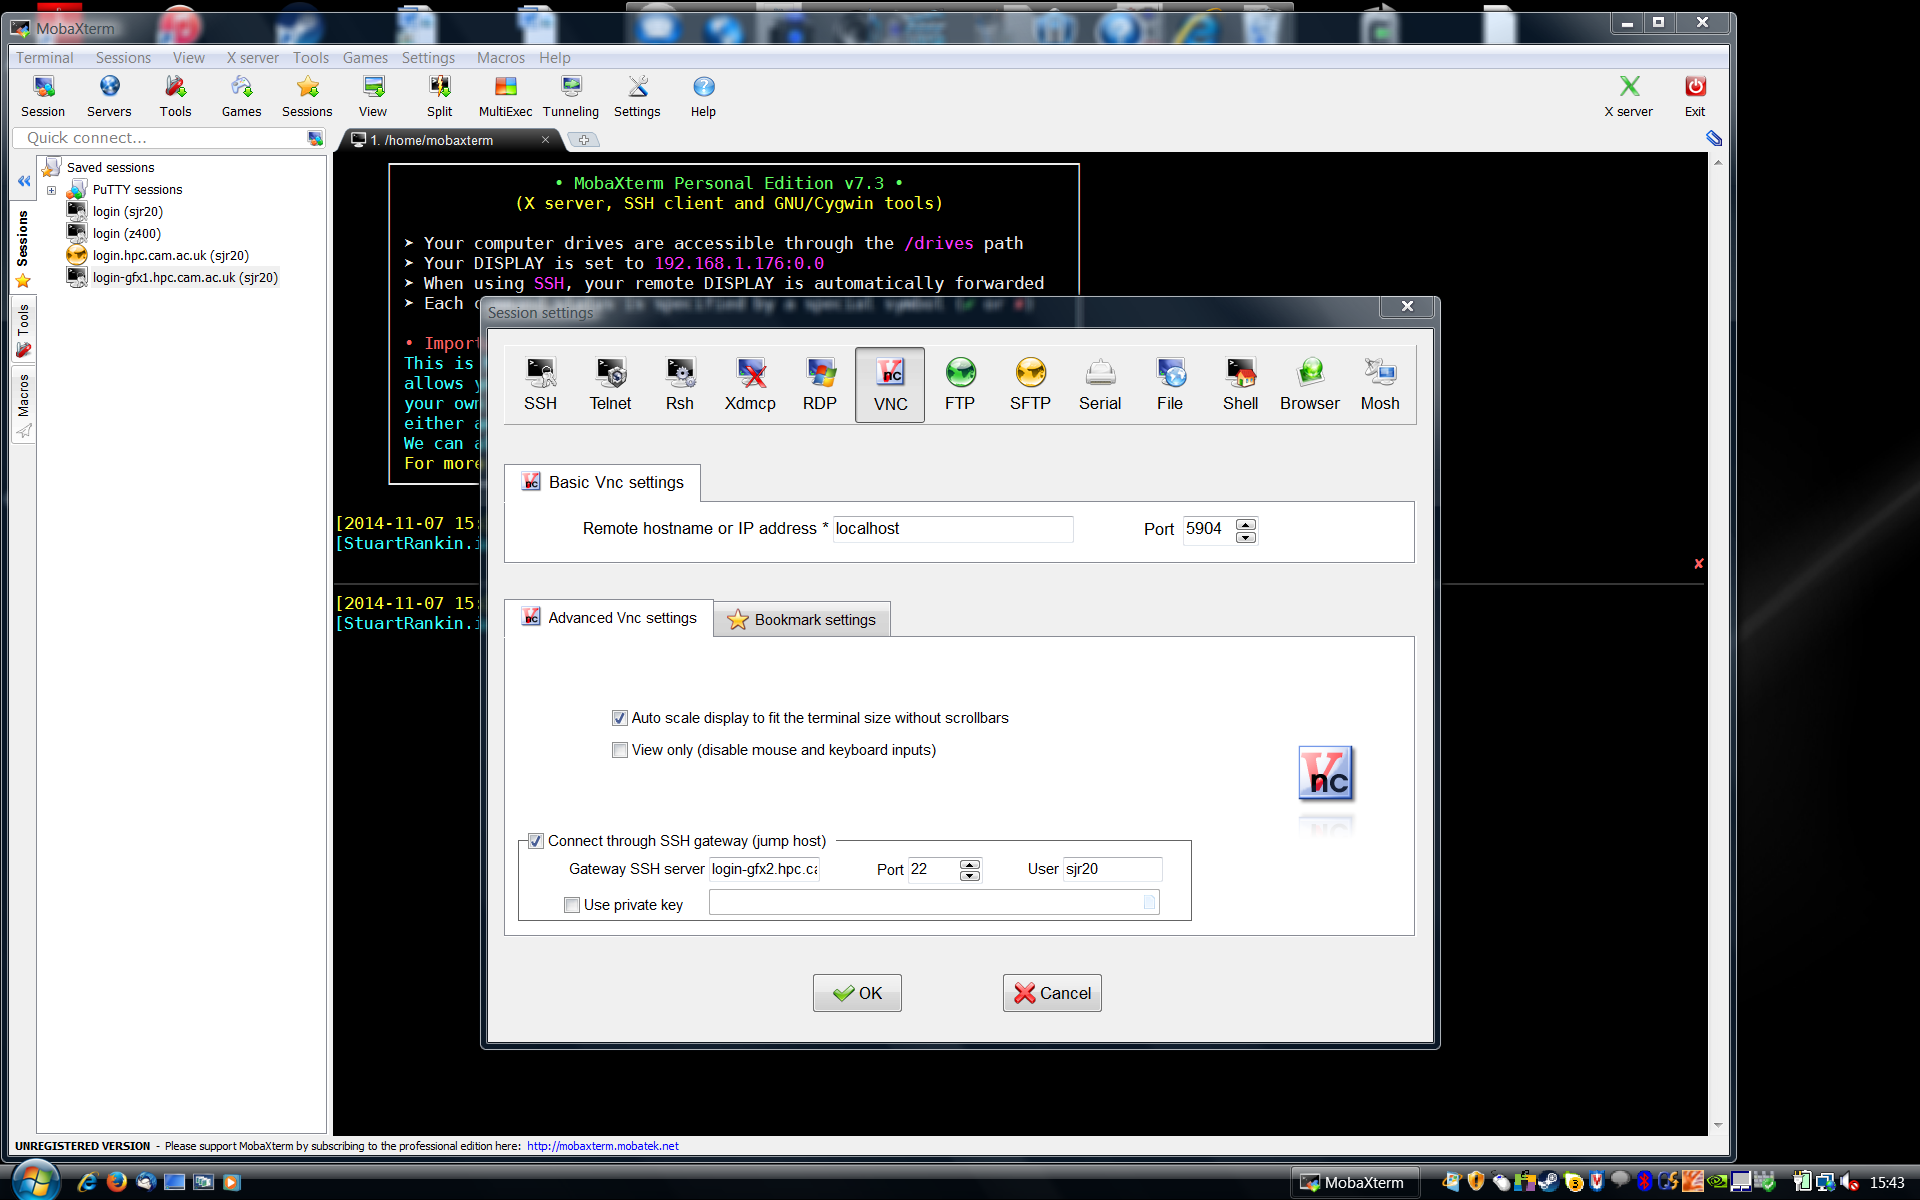
\includegraphics[height=0.8\textheight]{imgs/mobaxterm-turbovnc.png}}
\end{center}
\end{frame}

\section{User Environment}
\begin{frame}{Using HPC: User Environment}
\begin{itemize}
\item<1,3->{\visible<1>{CentOS Linux 7.4 (}\alert<1>{{\color<3->{red}Red Hat Enterprise Linux 7}\visible<1>{.4 rebuild)}}}
\begin{itemize}
\item{\visible<1>{bash shell}}
\item{\visible<1>{Gnome or XFCE4 desktop \alert{(if you want)}}}
\item{\visible<1>{GCC compilers and other development software.}}
\end{itemize}
\item<2->{But you don't need to know that.}
\end{itemize}
\end{frame}

\subsection{Filesystems}
\begin{frame}{User Environment: Filesystems}
When you apply for an HPC account a home directory is created for you. 
\begin{itemize}
\item{\alert{/home/<crsid>}}
\begin{itemize}
\item{40GB quota.}
\item{Visible equally from all nodes.}
\item{Single storage server.}
\item{Hourly, daily, weekly snapshots copied to tape.}
\item{Not intended for job outputs or large/many input files.}
\end{itemize}
\item{\alert{/rds/user/<crsid>/hpc-work}}
\begin{itemize}
\item{Visible equally from all nodes.}
\item{Larger and faster, 1TB quota plus a 1 million file limit).}
\item{Intended for job inputs and outputs.}
\item{{\color{red}Not backed up.}}
 \pause
\end{itemize}
\end{itemize}
\end{frame}

\begin{frame}[fragile]{Filesystems: Quotas}
\begin{itemize}
\item{quota}
\begin{semiverbatim}
\tiny
[sjr20@login-a-1 ~]\$ quota -s
Disk quotas for user sjr20 (uid 1004): 
     Filesystem   space   quota   limit   grace   files   quota   limit   grace
10.44.82.252:/hpc-work
                     0K   1024G   1126G               1       0       0        
10.44.82.252:/home
                 13272K  51200M  56320M             345       0       0        
\end{semiverbatim}
\item<1-|handout:1->{\alert{Aim to stay below the soft limit (\emph{quota}).}}
\item<2-|handout:1->{\alert{Once over the soft limit, you have 7 days grace to return below.}}
\item<3-|handout:2>{\alert{When the grace period expires, or you reach the hard limit (\emph{limit}), no more data can be written.}}
\item<4-|handout:2>{\alert{It is important to rectify an out of quota condition ASAP.}}
\end{itemize}
\end{frame}

\subsection{Exceeding 1TB of scratch}
\begin{frame}{Our storage services}
\begin{itemize}
\item{We have several storage services for users that need to exceed 1TB.}
\pause
\item{\alert{http://www.uis.cam.ac.uk/initiatives/storage-strategy/storage-services}}
\item{The most relevant services to HPC are RCS and RDS.}
\item{RCS - Research Cold Store is for data that isn't changing, data goes to disk then two sets of tapes.}
\item{RDS - Research Data Store, non backed up high performance storage for projects.}
\end{itemize}
\end{frame}

\begin{frame}[fragile]{Filesystems: Quotas}
\begin{itemize}
\item{quota}
\begin{semiverbatim}
\tiny
====================================================================================
Usage on /rds (lfs quota -u abc123 /rds):
====================================================================================
Disk quotas for user abc123 (uid 456):
      Filesystem  kbytes   quota   limit   grace   files   quota   limit   grace
 /rds/abc123 \only<1|handout:1>{9298708}\only<2-|handout:2->{{\color{red}*1073742000}}  1073741824 1181116006   -   165588       0       0       -
...
\end{semiverbatim}
\item<1-|handout:1->{\alert{Aim to stay below the soft limit (\emph{quota}).}}
\item<2-|handout:1->{\alert{Once over the soft limit, you have 7 days grace to return below.}}
\item<3-|handout:2>{\alert{When the grace period expires, or you reach the hard limit (\emph{limit}), no more data can be written.}}
\item<4-|handout:2>{\alert{It is important to rectify an out of quota condition ASAP.}}
\end{itemize}
\end{frame}

\begin{frame}{Filesystems: Backups}
\begin{itemize}
\item<1->{Disk snapshots and tape (as of May 2017).}
\item<2->{{\color{red}They are not an undelete - take care when deleting.}}
\item<3->{Successful restoration depends on:}
\begin{itemize}
\item{The file having existed long enough to have been backed up at all.}
\item{The last good version existing in a current backup.}
\item<4->{\color{red}Request restoration as soon as possible with \emph{location} and \emph{exact time of loss}.}
\medskip
\visible<5->{\item{\color{purple}\huge Scratch files are not backed up.}}
\end{itemize}
\end{itemize}
\end{frame}

\begin{frame}{Filesystems: Automounter}
\begin{itemize}
\item{Directories under /scratch are \alert{automounted}.}
\item{They only appear under /scratch when explicitly referenced.}
\item{Thus when browsing /scratch may appear too empty\hfill\\
\qquad\alert{--- use \emph{ls} or \emph{cd} to reference /scratch/abc123 explicitly.}}
\end{itemize}
\end{frame}

\begin{frame}{Filesystems: Permissions}
\begin{itemize}
\item{\color{red}Be careful and if unsure, please ask support.}
\begin{itemize}
\item{Can lead to \alert{accidental destruction} of your data or \alert{account compromise}.}
\end{itemize}
\item{Avoid changing the permissions on your home directory.}
\begin{itemize}
\item{Files under /home are particularly security sensitive.}
\item{Easy to break passwordless communication between nodes.}
\end{itemize}
\end{itemize}
\end{frame}

\subsection{Software}
\begin{frame}{User Environment: Software}
\begin{itemize}
\item{Free software accompanying \alert{Red Hat Enterprise Linux} is (or can be) provided.}
\item{Other software (free and non-free) is available via \alert{modules}.}
\item{Proprietary software currently available includes Matlab and COMSOL.}
\item{New software may be possible to provide on request.}
\item{\alert{Self-installed software should be properly licensed.}}
  \pause
\item{\color{red}\emph{sudo will not work.}\/ (You should be worried if it did.)}
\end{itemize}
\end{frame}

\subsection{Environment Modules}
\begin{frame}[fragile]{User Environment: Environment Modules}
\begin{itemize}
\item{Modules load or unload additional software packages.}
\item{Some are \alert{required} and automatically loaded on login.}
\item{Others are optional extras, or possible replacements for other modules.}
\item{\alert{Beware} unloading default modules in $\tilde{}\text{/.bashrc}$.}
\item{\alert{Beware} overwriting environment variables such as PATH and LD\_LIBRARY\_PATH in $\tilde{}\text{/.bashrc}$. If necessary append or prepend.}
\end{itemize}
\end{frame}

\subsection{Environment Modules}
\begin{frame}[fragile]{User Environment: Environment Modules}
\begin{itemize}
\item{Currently loaded:}
\begin{semiverbatim}
\scriptsize
module list
Currently Loaded Modulefiles:
  1) dot                     3) centos7/global
  2) slurm                   4) centos7/default-basic
\end{semiverbatim}
\medskip
\item{Available:}
\begin{semiverbatim}
\scriptsize
module av
\end{semiverbatim}
\end{itemize}
\end{frame}

\begin{frame}[fragile]{User Environment: Environment Modules}
\begin{itemize}
\item{Whatis:}
\begin{semiverbatim}
\tiny
module whatis openmpi-3.0.0-gcc-4.8.5-n2hvjgm
openmpi-3.0.0-gcc-4.8.5-n2hvjgm: The Open MPI Project is an open source...
\end{semiverbatim}
\medskip
\item{Load:}
\begin{semiverbatim}
\scriptsize
module load openmpi-3.0.0-gcc-4.8.5-n2hvjgm
\end{semiverbatim}
\medskip
\item{Unload:}
\begin{semiverbatim}
\scriptsize
module unload openmpi-3.0.0-gcc-4.8.5-n2hvjgm
\end{semiverbatim}
\end{itemize}
\end{frame}

\begin{frame}[fragile]{User Environment: Environment Modules}
\begin{itemize}
\item{Matlab}
\begin{semiverbatim}
\scriptsize
module load matlab/r2018a
\end{semiverbatim}
\medskip\pause
\item{Invoking matlab in batch mode:\hfill\\
  \qquad \alert{matlab -nodisplay -nojvm -nosplash command}\hfill\\
  where the file \alert{command.m} contains your matlab code.}
  \pause
  \item{The current site license contains the Parallel Computing Toolbox.}
\end{itemize}
\end{frame}

\begin{frame}[fragile]{User Environment: Environment Modules}
\begin{itemize}
\item{Purge:}
\begin{semiverbatim}
\scriptsize
module purge
\end{semiverbatim}
\smallskip
\item{Defaults:}
\begin{semiverbatim}
\scriptsize
module show centos7/default-basic
module load centos7/default-basic
\end{semiverbatim}
\medskip
\item{Run time environment must match compile time environment.}
\end{itemize}
\end{frame}

\subsection{Compilers}
\begin{frame}[fragile]{User Environment: Compilers}
  \begin{itemize}
    \item{GCC}
\begin{semiverbatim}
\scriptsize
gcc -O3 -mtune=native code.c -o prog
gfortran -O3 -mtune=native code.f90 -o prog
\medskip
module load openmpi-3.0.0-gcc-4.8.5-n2hvjgm
mpicc -O3 -mtune=native mpi_code.c -o mpi_prog
mpif90 -O3 -mtune=native mpi_code.f90 -o mpi_prog
\end{semiverbatim}
\pause
\item{Exercise 5: Modules and Compilers}
\end{itemize}
\end{frame}


%15:00
%Break
%15:15

\section{Job Submission}
\begin{frame}{Using HPC: Job Submission}
\centerline{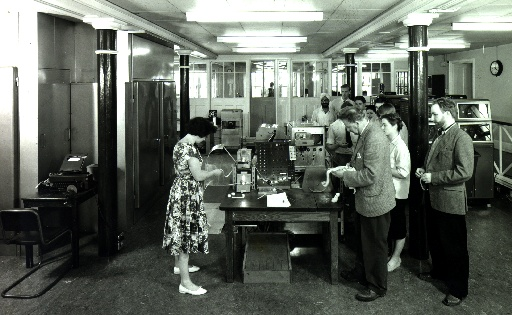
\includegraphics[width=1\textwidth]{imgs/EDSAC_2_1960.jpg}}
\end{frame}
\begin{frame}{Using HPC: Job Submission}
\begin{itemize}
\item{Compute resources are managed by a scheduler:\hfill\\\qquad\alert{SLURM}/PBS/SGE/LSF/\ldots}
\item{Jobs are submitted to the scheduler\hfill\\\qquad --- analogous to submitting jobs to a print queue\hfill\\\qquad --- a file (\emph{submission script}) is copied and queued\hfill\\\qquad \hphantom{---} for processing.}
\end{itemize}
\end{frame}

\begin{frame}{Using HPC: Job Submission}
\begin{itemize}
\item{Jobs are submitted from the \alert{login node}\hfill\\\qquad  --- not itself managed by the scheduler.}
\item{Jobs may be either non-interactive (\alert{batch}) or \alert{interactive}.}
\pause
\item{\alert{Batch} jobs run a shell script on the first of a list of allocated nodes.}
\item{\alert{Interactive} jobs provide a command line on the first of a list of allocated nodes.}
\end{itemize}
\end{frame}

\begin{frame}{Using HPC: Job Submission}
\begin{itemize}
\item{Jobs may use \alert{part} or \alert{all} of one or more nodes\hfill\\
\qquad --- the owner can specify \mbox{\tt --exclusive} to force exclusive\hfill\\\qquad\hphantom{---} node access.}
\item{Template submission scripts are available under\hfill\\
\qquad \alert{$\tilde{}$/job\_templates}.}
\end{itemize}
\end{frame}

\begin{frame}[fragile]{Job Submission: Using SLURM}
\begin{itemize}
\item{Prepare a shell script and submit it to SLURM:}
\begin{semiverbatim}
\scriptsize
[abc123@login-a-1]$ sbatch slurm_submission_script
Submitted batch job {\color{red}790299}
\end{semiverbatim}
\end{itemize}
\end{frame}

\begin{frame}[fragile]{Job Submission: Show Queue}
\begin{itemize}
\item{Submitted job scripts are copied and stored in a queue:}
\begin{semiverbatim}
\tiny
[abc123@login-a-1]$ squeue -u abc123
             JOBID PARTITION     NAME     USER ST       TIME  NODES NODELIST(REASON)
            {\color{red}790299}   skylake     Test3  abc123 PD       0:00      2 (\only<1>{{\color{blue}Priority}}\only<2>{{\color{green}Resources}}\only<3>{{\color{red}AssocGrpCPUMinsLimit}})
            790290   skylake     Test2  abc123  R   27:56:10      2 cpu-a-[1,10]
\end{semiverbatim}
\end{itemize}
\end{frame}

\begin{frame}[fragile]{Job Submission: Monitor Job}
\begin{itemize}
\item{Examine a particular job:}
\begin{semiverbatim}
\scriptsize
[abc123@login-a-1]$ scontrol show job={\color{red}790290}
\end{semiverbatim}
\end{itemize}
\end{frame}

\begin{frame}[fragile]{Job Submission: Cancel Job}
\begin{itemize}
\item{Cancel a particular job:}
\begin{semiverbatim}
\scriptsize
[abc123@login-a-1]$ scancel {\color{red}790290}
\end{semiverbatim}
\end{itemize}
\end{frame}

\begin{frame}[fragile]{Job Submission: Scripts}
\begin{itemize}
\item{SLURM\hfill\\
In \alert{$\tilde{}$/job\_templates}, see examples: \alert{slurm\_submit.skylake.generic}, \alert{slurm\_submit.skylake.matlab}.}
  
\begin{semiverbatim}
\tiny
#!/bin/bash
#! Name of the job:
{\color<2->{red}#SBATCH} -J myjob
#! Which project should be charged:
{\color<2->{red}#SBATCH} -A NPL-GENERAL-CPU
#! How many whole nodes should be allocated?
{\color<2->{red}#SBATCH} --nodes=1
#! How many tasks will there be in total? (<= nodes*32)
{\color<2->{red}#SBATCH} --ntasks={\color<3->[rgb]{1,0,0}\only<1-3>{1}\only<4->{16}}
#! How much wallclock time will be required?
{\color<2->{red}#SBATCH} --time=02:00:00
#! Select partition:
{\color<2->{red}#SBATCH} -p skylake
...
\end{semiverbatim}
\item<2->{{\color{red}\#SBATCH} lines are \emph{structured comments}\hfill\\
\qquad --- correspond to sbatch command line options.}
\item<3->{\alert{The above job will be given {\color<3->[rgb]{1,0,0}\only<1-3>{1 cpu}\only<4->{16 cpus}} on 1 node for 2 hours (by default there is 1 task per node, and 1 cpu per task).}}
\end{itemize}
\end{frame}

\begin{frame}[fragile]{Job Submission: Accounting Commands}
\begin{itemize}
\item{How many core hours available do I have?}
\begin{semiverbatim}
\tiny
mybalance

User           Usage |        Account     Usage | Account Limit Available (hours)
---------- --------- + -------------- --------- + ------------- ---------
sjr20              3 |    SUPPORT-CPU     2,929 |    22,425,600 {\color{red}22,422,671}
sjr20              0 |    SUPPORT-GPU         0 |        87,600    {\color{red}87,600}
\end{semiverbatim}
\smallskip
\item{How many core hours does some other project or user have?}
\begin{semiverbatim}
\tiny
gbalance -p SUPPORT-CPU

User           Usage |        Account     Usage | Account Limit Available (hours)
---------- --------- + -------------- --------- + ------------- ---------

pfb29          2,925 |    SUPPORT-CPU     2,929 |    22,425,600 22,422,671
sjr20 *            3 |    SUPPORT-CPU     2,929 |    22,425,600 22,422,671
...
(Use -u for user.)
\end{semiverbatim}
\smallskip
\item{List all jobs charged to a project/user between certain times:}
\begin{semiverbatim}
\Tiny
gstatement -p NPL-GENERAL-CPU  -u xyz10 -s "2018-04-01-00:00:00" -e "2018-04-30-00:00:00" 
       JobID      User    Account    JobName  Partition                 End ExitCode      State  CompHrs 
------------ --------- ---------- ---------- ---------- ------------------- -------- ---------- -------- 
263              xyz10 support-c+ _interact+    skylake 2018-04-18T19:44:40      0:0    TIMEOUT      1.0
264              xyz10 support-c+ _interact+    skylake 2018-04-18T19:48:07      0:0 CANCELLED+      0.1
275              xyz10 support-c+ _interact+    skylake             Unknown      0:0    RUNNING      0.3
...
\end{semiverbatim}
\end{itemize}
\end{frame}


\subsection{Single Node Jobs}
\begin{frame}[fragile]{Job Submission: Single Node Jobs}
\begin{itemize}
\item{Serial jobs requiring large memory, or OpenMP codes.}
\begin{semiverbatim}
\scriptsize
#!/bin/bash
\ldots
#SBATCH --nodes=1
\uncover<2-|handout:2->{{\color{red}#SBATCH --ntasks=1
# Default is 1 task per node}} 
\uncover<3-|handout:2->{{\color{red}#SBATCH --cpus-per-task=\only<3-5|handout:2>{1}\only<6,8-|handout:3,5->{32 # Whole node}\only<7|handout:4>{16  # Half node}
\only<3-5|handout:2>{# Default is 1 cpu (core) per task}}}
\uncover<4-5|handout:2>{{\color{red}#SBATCH --mem=5990
# Memory per node in MB - default is pro rata by cpu number}}
\uncover<5|handout:2>{{\color{red}# Increasing --mem or --cpus-per-task implicitly increases the other}}
\ldots
\uncover<6-|handout:3->{{\color{red}export OMP\_NUM\_THREADS=\only<6|handout:3>{32}\only<7-|handout:4->{16}  # For OpenMP across \only<6|handout:3>{32}\only<7-|handout:4->{16} cores\only<8-|handout:5->{ (using all memory)}}}
$application \$options
\ldots
\end{semiverbatim}
\end{itemize}
\end{frame}

\subsection{MPI Jobs}
\begin{frame}[fragile]{Job Submission: MPI Jobs}
\begin{itemize}
\item{Parallel job across multiple nodes.}
\begin{semiverbatim}
\scriptsize
#!/bin/bash
\ldots
#SBATCH --nodes={\color{red}4}
#SBATCH --ntasks=\alert{\only<1|handout:1>{128}\only<2-|handout:2->{64}}     # \only<1|handout:1>{i.e.\ {\color[rgb]{0,0.8,0}32}}\only<2-|handout:2->{i.e.\ {\color[rgb]{0,0.8,0} 16}}x{\color{red}4} MPI tasks in total.
\uncover<2-|handout:2->{{\color{red}#SBATCH --cpus-per-task=2}}
\ldots
mpirun\only<2-|handout:2->{ -ppn {\color[rgb]{0,0.8,0}16}} -np \alert{\only<1|handout:1>{128}\only<2-|handout:2->{64}} \$application \$options
\ldots
\end{semiverbatim}
\item<3-|handout:2->{\small SLURM-aware MPI launches remote tasks via SLURM.}
\item<3-|handout:2->{\small The template script uses \$SLURM\_TASKS\_PER\_NODE to set PPN.}
\end{itemize}
\end{frame}

\subsection{Hybrid Jobs}
\begin{frame}[fragile]{Job Submission: Hybrid Jobs}
\begin{itemize}
\item{Parallel jobs using both MPI and OpenMP.}
\begin{semiverbatim}
\scriptsize
#!/bin/bash
\ldots
#SBATCH --nodes={\color{red}4}
#SBATCH --ntasks=\alert{64}     # i.e.\ {\color[rgb]{0,0.8,0}16}x{\color{red}4} MPI tasks in total.
#SBATCH --cpus-per-task={\color{brown}2}
\ldots
{\color{brown}export OMP\_NUM\_THREADS=2   # i.e.\ 2 threads per MPI task.}
mpirun -ppn {\color[rgb]{0,0.8,0}16} -np \alert{64} \$application \$options
\ldots
\end{semiverbatim}
\item<2->{\small This job uses \alert{128 CPUs} (each MPI task splits into 2 OpenMP threads).}
\end{itemize}
\end{frame}

\subsection{High Throughput Jobs}
\begin{frame}[fragile]{Job Submission: High Throughput Jobs}
\begin{itemize}
\item{Multiple serial jobs across multiple nodes.}
\item{Use \alert{srun} to launch tasks (\alert{job steps}) within a job.}
\begin{semiverbatim}
\scriptsize
#!/bin/bash
\ldots
#SBATCH --nodes=2
\ldots
cd directory\_for\_job1
\alert{srun} {\color<3>{red}--exclusive} {\color<2>{red}-N 1 -n 1} \$application \$options\_for\_job1 > output 2> err {\color<4>{red}&}
cd directory\_for\_job2
\alert{srun} {\color<3>{red}--exclusive} {\color<2>{red}-N 1 -n 1} \$application \$options\_for\_job2 > output 2> err {\color<4>{red}&}
...
cd directory\_for\_job64
\alert{srun} {\color<3>{red}--exclusive} {\color<2>{red}-N 1 -n 1} \$application \$options\_for\_job64 > output 2> err {\color<4>{red}&}
{\color<5>{red}wait}
\end{semiverbatim}
\item<6>{Exercise 6 - Submitting Jobs.}
\end{itemize}
\end{frame}

\subsection{Interactive Jobs}
\begin{frame}[fragile]{Job Submission: Interactive}
\begin{itemize}
\item{Compute nodes are accessible via SSH \alert{while you have a job running on them}.}
\pause
\item{Alternatively, submit an interactive job:}
\begin{semiverbatim}
\alert{sintr -A NPL-GENERAL-CPU -N1 -n8 -t 2:0:0}
\end{semiverbatim}
\medskip
\pause
\item{Within the window (screen session):}
\begin{itemize}
\item[$\ast$]{Launches a shell on the first node (when the job starts).}
\item[$\ast$]{Graphical applications should display correctly.}
\item[$\ast$]{Create new shells with \alert{ctrl-a c}, navigate with \alert{ctrl-a n} and \alert{ctrl-a p}.}
\item[$\ast$]{\alert{ssh} or \alert{srun} can be used to start processes on any nodes in the job.}
\item[$\ast$]{SLURM-aware MPI will do this automatically.}
\end{itemize}
\end{itemize}
\end{frame}


\subsection{Array Jobs}
\begin{frame}[fragile]{Job Submission: Array Jobs}
\begin{itemize}
\item{\alert{$http://slurm.schedmd.com/job\_array.html$}}
\item{Used for submitting and managing large sets of similar jobs.}
\item{Each job in the array has the same \alert{initial} options.}
\item{SLURM}
\begin{semiverbatim}
\scriptsize
[abc123@login-a-1]$ sbatch --array=\only<1,2>{{\color{red}1-7}}\only<2>{{\color{red}:2}}\only<3->{{\color{red}1,3,5,7}} -A NPL-GENERAL-CPU submit\_script
Submitted batch job {\color[rgb]{0,0.6,0}791609}
\tiny
\uncover<4->{[abc123@login-a-1]$ squeue -u abc123
             JOBID PARTITION     NAME     USER ST       TIME  NODES NODELIST(REASON)
          {\color[rgb]{0,0.6,0}791609}\_{\color{red}1} skylake      hpl    abc123  R       0:06      1 cpu-a-6
          {\color[rgb]{0,0.6,0}791609}\_{\color{red}3} skylake      hpl    abc123  R       0:06      1 cpu-a-16
          {\color[rgb]{0,0.6,0}791609}\_{\color{red}5} skylake      hpl    abc123  R       0:06      1 cpu-a-7
          {\color[rgb]{0,0.6,0}791609}\_{\color{red}7} skylake      hpl    abc123  R       0:06      1 cpu-a-7
}
\end{semiverbatim}
\uncover<5->{\centerline{{\color[rgb]{0,0.6,0}791609}\_{\color{red}1}, {\color[rgb]{0,0.6,0}791609}\_{\color{red}3}, {\color[rgb]{0,0.6,0}791609}\_{\color{red}5}, {\color[rgb]{0,0.6,0}791609}\_{\color{red}7}}}
\smallskip
\uncover<6->{\centerline{i.e.\ \$\{{\color[rgb]{0,0.6,0}SLURM\_ARRAY\_JOB\_ID}\}\_\$\{{\color{red}SLURM\_ARRAY\_TASK\_ID}\}}}
\smallskip
\uncover<7->{\leftline{\small SLURM\_ARRAY\_JOB\_ID${}={}$SLURM\_JOBID for the first element.}}
\end{itemize}
\end{frame}

\begin{frame}[fragile]{Job Submission: Array Jobs (ctd)}
\begin{itemize}
\item{Updates can be applied to specific array elements using \$\{{\color[rgb]{0,0.6,0}SLURM\_ARRAY\_JOB\_ID}\}\_\$\{{\color{red}SLURM\_ARRAY\_TASK\_ID}\}}
\item{Alternatively operate on the entire array via \$\{{\color[rgb]{0,0.6,0}SLURM\_ARRAY\_JOB\_ID}\}}.
\item{Some commands still require the SLURM\_JOB\_ID (sacct, sreport, sshare, sstat and a few others).}
\pause
\item{Exercise 7 - Array Jobs.}
\end{itemize}
\end{frame}

\subsection{Scheduling}
\begin{frame}{Scheduling}
\begin{itemize}
\item{SLURM scheduling is multifactor:}
  \pause
\begin{itemize}
\item{\alert{QoS} --- payer or non-payer?}
  \pause
\item{\alert{Age} --- how long has the job waited?\hfill\\\qquad
  \alert{Don't cancel jobs that seem to wait too long.}}
  \pause
\item{\alert{Fair Share} --- how much recent usage?\hfill\\\qquad
  \alert{Payers with little recent usage receive boost (not implemented yet).}}
  \pause
\item{\alert{sprio -j jobid}}
\end{itemize}
\pause
\item{\alert{Backfilling}}
\begin{itemize}
  \item{Promote lower priority jobs into gaps left by higher priority jobs.}
    \item{Demands that the higher priority jobs not be delayed.}
    \item{Relies on reasonably accurate wall time requests for this to work.}
      \item{Jobs of default length will not backfill readily.}
\end{itemize}
\end{itemize}
\end{frame}

\subsection{Wait Times}
\begin{frame}{Wait Times}
  \begin{itemize}
  \item{36 hour job walltimes are permitted.}
    \pause
  \item{\alert{This sets the timescale at busy times (\emph{without} backfilling).}}
    \pause
  \item{Use backfilling when possible.}
  \item{Short (1 hour or less) jobs have higher throughput.}
\end{itemize}
\end{frame}

\subsection{Checkpointing}
\begin{frame}{Checkpointing}
  \begin{itemize}
  \item{Insurance against failures during long jobs.}
  \item{Restart from checkpoints to work around finite job length.}
    \pause
  \item{Application native methods are best. Failing that $\ldots$}
  \end{itemize}
\end{frame}

\subsection{Scheduling Top Tips}
\begin{frame}{Job Submission: Scheduling Top Dos \& Don'ts}
\begin{itemize}
\item{\textbf{Do \ldots}}
\begin{itemize}
\item{Give reasonably accurate wall times (allows \alert{backfilling}).}
\item{Check your balance occasionally (\alert{mybalance}).}
\item{Test on a small scale first.}
\item{Implement \alert{checkpointing} if possible (reduces resource wastage).}
\end{itemize}
\medskip
\item{\textbf{Don't \ldots}}
\begin{itemize}
\item{Request more than you need\hfill\\
\qquad --- you will wait longer and use more credits.}
\item{Cancel jobs unnecessarily\hfill\\
\qquad ---  priority increases over time.}
\end{itemize}
\end{itemize}
\end{frame}

